\section{Protocols}
The IRMA Assurer protocol is an application level protocol. It is designed to run on top of TLS 1.2. Only the latest version of the TLS standard is considered cryptographically secure and therefore is the only version IRMA Assurer supports. A second argument for the use of version 1.2 is the possibility to achieve Perfect Forward Secrecy (PFS), meaning that in case the long term key is ever compromised, then the session keys derived from it before compromise are still secure~\cite{PFS}. This chapter will first describe the TLS protocol, explaining the chosen parameters. The IRMA Assurer protocol follows directly after.

\subsection{Transport Layer Security}
\begin{wrapfigure}{R}{0.45\textwidth}
  \centering
	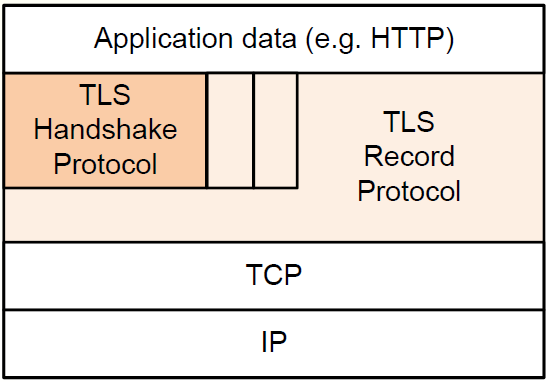
\includegraphics[width=0.4\textwidth]{images/tlsstack.png}
	\caption{TLS Protocol Hierarchy}
	\label{fig:tlsstack}
\end{wrapfigure}

The Transport Layer Security (TLS) protocol is a protocol operating on the presentation layer of the OSI Reference Model~\cite{osi}. It is a protocol that secures the connection between two parties across an insecure channel, ensuring secrecy~\cite{tls1.2}. It also has the possibility for authentication based on certificates. TLS is commonly used in web browsers to encrypt HTTP into HTTPS traffic, but it is capable of protecting any TCP connection~\cite{lecture}.

TLS 1.2 was defined in RFC 5246 in August 2008. It is based on the earlier TLS 1.1 specification. It was further refined in RFC 6176 in March 2011 removing their backward compatibility with SSL such that TLS sessions will never negotiate the use of Secure Sockets Layer (SSL) version 2.0.

\texttt{TLS vulnerable to handshake renegotiation attack, solved by RFC 5746~\cite{lecture}.}

The protocol consists of two major parts, TLS Handshake and TLS Record. Handshake is used for setting up connections between two parties, with optional authentication, while Record is used for ordering, encrypting and sending of the data. Handshake makes use of Record, so they work both alongside as well as on top of each other (see figure~\ref{fig:tlsstack}).



\subsubsection{TLS handshake}
Figure~\ref{fig:tlshandshake} shows a schematic overview of the TLS handshake, copied from RFC 5246~\cite{tls1.2}. The \texttt{*} indicates a step necessary for client-to-server authentication. The handshake begins when a client connects to a TLS-enabled server requesting a secure connection and presents a list of supported cipher suites (ciphers and hash functions). From this list, the server picks a cipher and hash function that it also supports and notifies the client of the decision. The server usually then sends back its identification in the form of a digital certificate. The certificate usually contains the server name, the trusted certificate authority (CA) and the server's public encryption key. The client may contact the server that issued the certificate (the trusted CA) and confirm the validity of the certificate before proceeding. In order to generate the session keys used for the secure connection, the client encrypts a random number with the server's public key and sends the result to the server. Only the server should be able to decrypt it, with its private key. From the random number, both parties generate a 'master secret' and then negotiate a session key for encryption and decryption.

The details about the underlying cryptographic functions selected for the IRMA Assurer protocol, such as encryption and hashing functions will be discussed later in section~\ref{sec:assumptions}.

\begin{verbbox}
Client                                               Server
------                                              -------
ClientHello              -------->
                                                ServerHello
                                               Certificate*
                                         ServerKeyExchange*
                                        CertificateRequest*
                         <--------          ServerHelloDone
Certificate*
ClientKeyExchange
CertificateVerify*
[ChangeCipherSpec]
Finished                 -------->
                                         [ChangeCipherSpec]
                         <--------                 Finished
Application Data         <------->         Application Data
\end{verbbox}

\begin{figure}[htb]
\centering
\theverbbox
\caption{TLS Handshake}
\label{fig:tlshandshake}
\end{figure}

\subsubsection{TLS record}
The record protocol handles the sending and receiving of TLS related messages. It forms the basis of the TLS protocol. When sending, it will split the data in blocks, optionally compress it, apply a MAC, encrypt the data, add a fragment header and finally send the data over TCP port 443. When receiving, it will decrypt the data, verify the MAC, optionally decompress, defragment and finally deliver the data to the upper layer. Essentially this protocol forms the secure channel between client and server~\cite{tls1.2}.

\subsection{IRMA Assurer}
The IRMA Assurer protocol makes use of TLS 1.2 as described above. This means both the server and the tablets will verify each other's certificates and agree upon a session key. Once a secure channel has been successfully set up, we have achieved privacy and data integrity of all communication over this channel~\cite{tls1.2}.

\subsection{Assumptions}
\label{sec:assumptions}
In this section we discuss the assumptions made with regard to Assurer. The section is divided into two parts. The first section discusses assumptions on the operational level and the second describes assumptions with respect to cryptography.

\subsubsection{Operational}
Operational assumptions mostly focus on procedures that have to be followed for the Assurer protocol to work. We reiterate some parts of the basic course of events described in section~\ref{subsec:bcoe} to make them explicit as assumptions. 

The entire ecosystem in which Assurer operates can be described as a star structure. At the center of the star will be the (only) server. The edges (points) of the star are formed by the clients. Clients do not communicate with each other, but only with the server. Each of these clients has their own NFC-enabled tablet, which is locked up in a safe and PIN code protected to prevent malicious use. By using an Android app installed on these tablets assurers may access data on passport chips and IRMA cards. Upon client initialization this app is installed on the tablet, as well as the DNS host name of the server. By using the host name the server has the option to switch IP addresses without breaking the system. Also installed on the tablet are a client certificate (signed by the server) required for authentication and its corresponding private key. The server checks the certificate for validity and also checks if it has not been revoked by accessing Certificate Revocation Lists (CRL), which mitigates issues with stolen tablets or misuse. Finally the public key of the server is installed for easy access.

Although subject to change, at the time of writing the communication between IRMA card and terminal, i.e. tablet, is still being sent in the clear. Upon reading data from a passport chip the integrity is verified by the client by executing BAC and PA, and sent to the server for further analysis. The server performs the same checks, plus AA, and looks up the person corresponding to the data in a central database. If everything is proven to be valid the server will create digitally signed attribute-based credentials that correspond to the passport data. The server will then send these ABCs to the client, who will in turn install them on the person's IRMA card. Upon successful installation onto the IRMA card, the ABCs are securely deleted from both server and client. Furthermore, the passport data is securely deleted from the server and client. However the server does keep a log of the BSN that was part of the attribute signing request sent by the client, along with a timestamp. This facilitates traceability in case of anomalies. Finally, we do not support TLS session resuming. This property allows clients to send a stored session identifier to the server and then pick up where left off. Supporting this weakens the strength of the TLS connection, in particular the PFS property of TLS.\footnote{\url{https://timtaubert.de/blog/2014/11/the-sad-state-of-server-side-tls-session-resumption-implementations/}} Since we wish to have PFS we do not allow session resuming.

\subsubsection{Cryptographic}
Before going into the cryptographic choices regarding Assurer it is important to take a quick look at the transport layer used below. There are two options, the User Datagram Protocol (UDP) and the Transport Control Protocol (TCP). We have chosen to make use of TCP for its transport layer protocol. The main reason for this is that we require the packets to be delivered without packet loss. In other words, we favor TCP over UDP for its high reliability. Furthermore it is best compatible with the TLS protocol which we aim to use. Other arguments for choosing TCP include its data flow control and packet reordering capabilities.

In order to achieve the goals described in section~\ref{sec:goals} several choices have been made regarding the cryptography. What follows is an argumentation for the decisions made for Assurer. 

The guideline for choosing supported cipher suites is to offer perfect forward secrecy. Any cipher suites that offer PFS capabilities have been selected, while suites that do not are not selected. In principle, any public key encryption scheme can be used to build a key exchange with PFS by using the encryption scheme with ephemeral public and private keys~\cite{PFS}. This means we have the option to use any public key infrastructure as long as we throw away the keys when we're done using them. Furthermore we can either choose elliptic curve cryptography or conventional cryptography. Because we wish to achieve mutual authentication both parties need to exchange certificates. These certificates must be of type X.509v3 in accordance with the TLS specifications~\cite{tls1.2}. The type of cryptography used for these certificates may either be RSA or DSA. Generally, in terms of performance, neither is significantly better than the other, meaning we may support both. 

As explained above we have chosen TLS 1.2 for its resistance against publicly known feasible attacks, as well as for its Perfect Forward Secrecy capabilities. This requires that the key generation for the encryption scheme must be fast enough. For most applications this disqualifies, for example, the use of ephemeral RSA public key encryption for achieving PFS, since the latter requires the generation of two long prime numbers for each exchange, a relatively costly operation~\cite{PFS}. For this reason we have selected the Diffie-Hellman Key Exchange protocol. Furthermore because of the faster key generation, better performance and shorter key length while still achieving the same level of security we have chosen to use elliptic curves.\footnote{\url{https://www.nsa.gov/business/programs/elliptic_curve.shtml}}

Since the Assurer protocol is to be used only on newly developed hardware and software it is safe to use the newest cryptography; there should not be any compatibility issues. Mozilla lists the following as the best choice for modern clients in their documentation on server-side TLS,\footnote{\url{https://wiki.mozilla.org/Security/Server_Side_TLS}} ordered from most recommended to least recommended (the $!$ indicates forbidden):

\begin{description}
	\item [Ciphersuite] \texttt{ECDHE-RSA-AES128-GCM-SHA256, ECDHE-ECDSA-AES128-GCM-SHA256, \\
ECDHE-RSA-AES256-GCM-SHA384, ECDHE-ECDSA-AES256-GCM-SHA384, \\
DHE-RSA-AES128-GCM-SHA256, DHE-DSS-AES128-GCM-SHA256, kEDH+AESGCM, \\
ECDHE-RSA-AES128-SHA256, ECDHE-ECDSA-AES128-SHA256, \\
ECDHE-RSA-AES128-SHA, ECDHE-ECDSA-AES128-SHA, \\
ECDHE-RSA-AES256-SHA384, ECDHE-ECDSA-AES256-SHA384, \\
ECDHE-RSA-AES256-SHA, ECDHE-ECDSA-AES256-SHA, DHE-RSA-AES128-SHA256, \\
DHE-RSA-AES128-SHA, DHE-DSS-AES128-SHA256, DHE-RSA-AES256-SHA256, \\
DHE-DSS-AES256-SHA, DHE-RSA-AES256-SHA, !aNULL, !eNULL, !EXPORT, \\
!DES, !RC4, !3DES, !MD5, !PSK}
  \item [Versions] \texttt{TLSv1.1, TLSv1.2}
  \item [RSA key size] \texttt{2048}
  \item [DH Parameter size] \texttt{2048}
  \item [Elliptic curves] \texttt{secp256r1, secp384r1, secp521r1} (at a minimum)
  \item [Certificate signature] \texttt{SHA-256}
  \item [HSTS] \texttt{max-age=15724800}
\end{description}

Note that this is the optimal configuration for Mozilla's own servers providing HTTPS connections, which explains the mention of HSTS. For the Assurer protocol we are only interested in cipher suites supported in TLS 1.2, while making use of elliptic curves and Diffie-Hellman, meaning we can safely ignore anything that is unrelated. Cross-referencing this list of cipher suites with the list of elliptic curve and TLS 1.2 cipher suites described by the OpenSSL documentation\footnote{\url{https://www.openssl.org/docs/apps/ciphers.html}} yields the following list of cipher suites supported by the IRMA Assurer protocol, in descending order of priority, named following IANA guidelines.\footnote{\url{http://www.iana.org/assignments/tls-parameters/tls-parameters.xhtml}} This naming convention differs from the one used by Mozilla, who use OpenSSL guidelines, but is in correspondence with the RFC documents on TLS. The blank lines indicate Mozilla favors either a non-elliptic curve or a TLS 1.2 incompatible cipher suite over the ones that follow. 

\begin{verbatim}
TLS_ECDHE_RSA_WITH_AES_128_GCM_SHA256
TLS_ECDHE_ECDSA_WITH_AES_128_GCM_SHA256
TLS_ECDHE_RSA_WITH_AES_256_GCM_SHA384
TLS_ECDHE_ECDSA_WITH_AES_256_GCM_SHA384

TLS_ECDHE_RSA_WITH_AES_128_CBC_SHA256
TLS_ECDHE_ECDSA_WITH_AES_128_CBC_SHA256

TLS_ECDHE_RSA_WITH_AES_256_CBC_SHA384
TLS_ECDHE_ECDSA_WITH_AES_256_CBC_SHA384
\end{verbatim}

There are many reasons for this particular ordering. We highlight the main reasons below. 

\begin{itemize}
  \item ECDHE+AESGCM ciphers are selected first. These are TLS 1.2 ciphers and not widely supported at the moment. No known attack currently targets these ciphers.
  \item PFS ciphersuites are preferred, with ECDHE first, then DHE.
	\item ECDHE provides faster handshakes than DHE.\footnote{\url{http://vincent.bernat.im/en/blog/2011-ssl-perfect-forward-secrecy.html}}~\cite{pfsprice}.
  \item AES 128 is preferred to AES 256, because it provides good security, is really fast, and seems to be more resistant to timing attacks.
  \item SHA256 is favored over SHA384. This appears to be mainly for interoperability purposes.
\end{itemize}

Galois Counter Mode (GCM) is an Authenticated Encryption (AE) algorithm. AE algorithms are designed to provide both data authenticity (integrity) and confidentiality. Since both are goals of Assurer we favor GCM over CBC, but do not require it.

For more information about the reasons behind this ordering please see~\cite{mozilla}.

\subsubsection{DH parameters}
Unfortunately, some widely used clients lack support for ECDHE and must then rely on DHE to provide perfect forward secrecy. This is true for Android $< 3.0.0$, Java $< 7$ and OpenSSL $< 1.0.0$, among others. Nowadays many, if not all, devices run Android versions higher than 3.0.0, so we don't expect to see issues here. However the Java requirement could lead to issues when implementing Assurer as an Android app, mainly because of the many IRMA-related dependencies that such an app has to deal with. These dependencies may not support Java 7 or 8 yet. Adding to that, Java 6 and 7 do not support Diffie-Hellman parameters larger than 1024 bits. This has consequences for the PFS requirement of Assurer. The only way a secure connection can be achieved from a Java 6 client is to use DHE cipher suites and use 1024-bit groups.

Use of the most widely used 1024-bit pre-computed Oakley group 2, standardized in~\cite{ike}, is considered unsafe, mainly because it is very likely that a state-level adversary may have broken it. In any case it is recommended to generate a random DH group instead of using a standardized one when setting up a new server~\cite{logjam}.

CBC ciphers can be attacked with the Lucky Thirteen attack\footnote{\url{http://www.isg.rhul.ac.uk/tls/Lucky13.html}} if the library is not written carefully to eliminate timing side channels. This attack requires multiple sessions and is possibly detectable due to the low volume of traffic in the IRMA Assurer protocol.

\paragraph{Logjam}
When choosing this list of supported cipher suites we have chosen the ``modern'' preset described by Mozilla. This is especially important, because of the recently discovered Logjam attack on the Diffie-Hellman key agreement, in particular within TLS, SSH and VPN connections~\cite{logjam}. Essentially Logjam is a type of attack that allows an attacker to downgrade the security of the connection to DHE export cipher suites. It is also possible to attack weak ($\leq$ 1024-bit) Diffie-Hellman groups by precomputing the group and then using it for lookups. The short term solution for mitigating Logjam attacks is for servers to disable export ciphers and use freshly generated groups of 2048 bits or larger. Clients should no longer accept groups of sizes lower than 1024 bits. In the long term however it is preferable to switch to elliptic curve cryptography (ECC) and not allow any other cipher suites. This is because none of the attacks presented work against ECC. As described above the Assurer protocol only makes use of a subset of the ``modern'' preset, which in turn only makes use of ECC cipher suites, and therefore is not susceptible to the Logjam attack.

\paragraph{Elliptic curves}
NIST has defined 15 standard curves~\cite{dss}. However, in practice, many implementations only support two of them, P-256 and P-384, because that's what the NSA recommends. As seen above Mozilla recommends to use at the very least P-256, P-384 and P-521. For Assurer we will follow that recommendation.

\subsubsection{Certificates}
\begin{itemize}
	\item Each client posesses one certificate, signed by the server, with which it may authenticate to the server. This occurs during the run of the TLS handshake protocol.
  \item Each passport contains one certificate with which the authenticity may be verified (see section~\ref{subsec:passports}).
\end{itemize}

\subsubsection{Keys}
The server owns two keypairs. The first keypair is used for signing and verification of certificates while the second one is used for the issuing and verification of attribute based credentials. A client only owns one keypair, which is used for signing and verification of certificates. The server's public key used for signing and verification is pre-loaded onto the clients during initialization, while the clients' public keys are stored within the pre-loaded certificates.

The use of TLS 1.2 with the aforementioned cryptographic options for the handshake will result in a symmetric session key held by both parties. From this point onwards we therefore have a secure channel to use for application data transfer.

\subsubsection{Application data}
All application data is protected with the session key as generated by the TLS handshake protocol. 

\ldots


\subsubsection{Final remarks}
\begin{itemize}
  \item 
\end{itemize}


